\section{Additional results}
\label{app:more}

\begin{figure}[!htb]
\centering
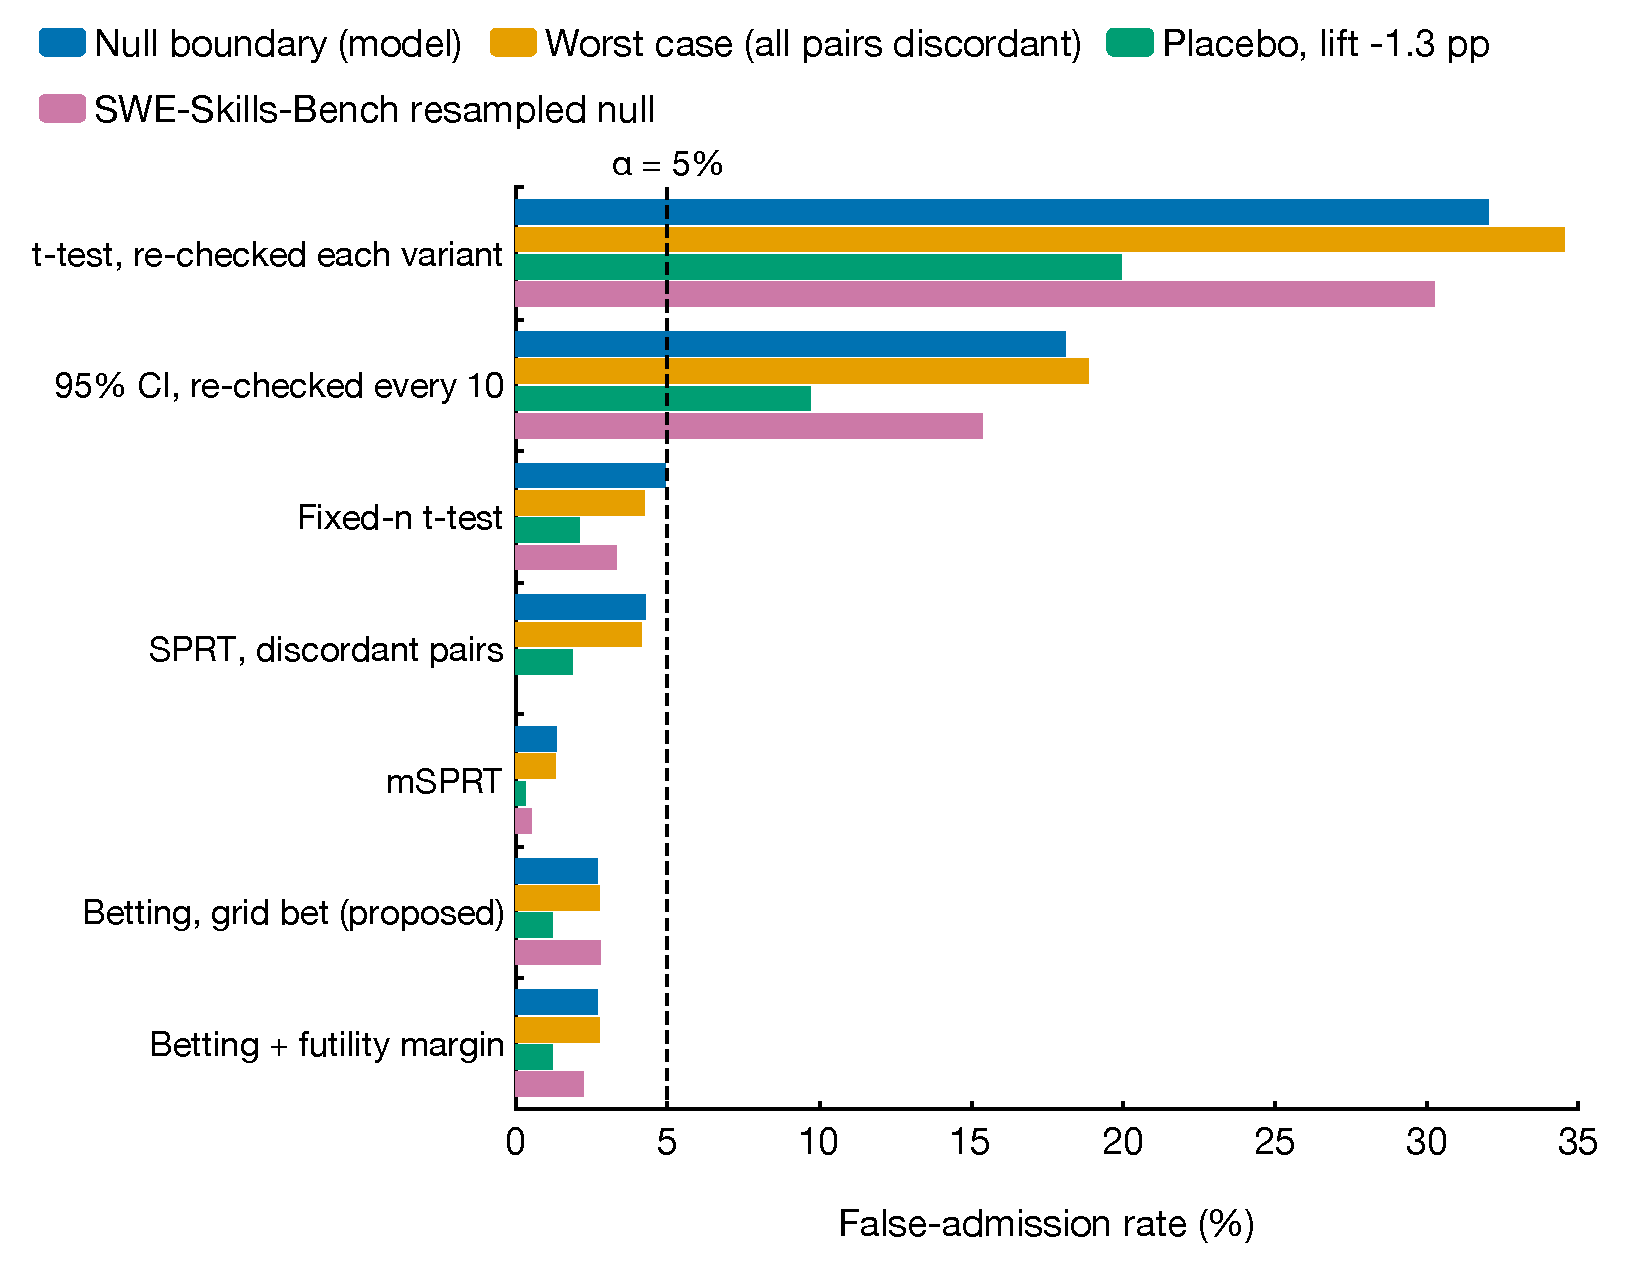
\includegraphics[width=0.64\linewidth]{F2_false_admission.pdf}
\caption{False-admission rate under nulls (E1, E8). Model nulls use \PReps{} replicates each; the SWE-Skills-Bench resampled null draws differences from the released data with random signs. The SPRT is defined only for pass/fail data and is not run on the batch pass rates of SWE-Skills-Bench. Dashed line: $\alpha=5\%$.}
\label{fig:false}
\end{figure}

\paragraph{Validity checks.} Validity also holds for strong and weak common random numbers, for $r=3$ attempts per arm, and for a margin $\delta=0.05$. The released SWE-Skills-Bench data are tie-heavy, which makes the exact sign-flip test conservative; on continuous data the per-configuration rate would be near 5\% and the any-of-four rate near 19\% (\NShopRatio-fold on the released data). A one-sided version of the source rule marks \NSweOneSided{} cells.

\paragraph{Departures from the conditional null (E21).} E21 simulates exams of a useless skill ($\Delta=0$ before any departure, $\delta=0$) under each departure listed in Section~\ref{sec:discussion}, with 20{,}000 exams per cell (Monte Carlo standard error at most 0.4 points) and the default outcome model. The exam-level coin fixes the lift of a whole exam at $\pm s$; a model change at a uniform variant index shifts both arms' logits by $\pm1$, or the skill arm's by $\pm0.5$; shared effects add a normal logit effect to the skill arm, common to blocks of variants, with the base lift re-solved so that the marginal lift stays zero; repeated seeds copy an earlier variant's outcome; and exclusion drops variants the skill arm lost, as if they were harness failures. Table~\ref{tab:nullstress} gives the false-admission rates. The fixed-$n$ $t$-test admits nothing under the hard coin because its statistic is undefined when every difference is equal.
\begin{table}[!htb]
\centering\small
\caption{False-admission rate (\%) of a useless skill under departures from the design (E21), target 5\%. Grid and PrPl use the futility margin.}
\label{tab:nullstress}
\begin{tabular}{lrrrrr}
\toprule
Departure from the design & Grid & PrPl & mSPRT & SPRT & Fixed-$n$ \\
\midrule
None (design of Section~\ref{sec:setup}) & 2.9 & 1.5 & 1.3 & 4.4 & 5.1 \\
Exam-level coin, $D_i\equiv\pm1$ & 49.4 & 49.4 & 49.4 & 49.4 & 0.0 \\
Exam-level coin, lift $\pm0.05$ & 22.2 & 26.0 & 23.6 & 20.2 & 17.8 \\
Exam-level coin, lift $\pm0.10$ & 49.3 & 49.5 & 49.5 & 41.7 & 40.1 \\
Model change mid-exam, both arms & 2.5 & 1.3 & 1.2 & 4.3 & 4.9 \\
Model change mid-exam, skill arm only & 15.5 & 14.4 & 17.4 & 7.7 & 7.3 \\
Shared effect, blocks of 5, sd 0.5 & 3.6 & 2.1 & 2.0 & 5.5 & 6.1 \\
Shared effect, blocks of 10, sd 0.5 & 5.1 & 3.1 & 3.0 & 7.0 & 6.9 \\
Shared effect, blocks of 10, sd 1.0 & 11.5 & 7.6 & 8.4 & 12.2 & 10.7 \\
Repeated seeds, 1\% & 2.9 & 1.6 & 1.4 & 4.5 & 5.0 \\
Repeated seeds, 5\% & 3.5 & 2.1 & 1.9 & 5.4 & 5.7 \\
Repeated seeds, 20\% & 7.4 & 5.2 & 4.7 & 9.7 & 9.4 \\
Excluding skill-arm losses, 1\% & 3.0 & 1.8 & 1.6 & 4.4 & 5.1 \\
Excluding skill-arm losses, 5\% & 3.7 & 2.4 & 2.1 & 5.9 & 6.4 \\
Excluding skill-arm losses, 20\% & 9.9 & 10.3 & 8.0 & 14.3 & 13.5 \\
\bottomrule
\end{tabular}

\end{table}

\paragraph{Total lineage cost (E19).} Theorem~\ref{thm:price} prices the helpful exam of a lineage under the lineage term alone. E19 measures the whole cost under the deployed level $\min(\alpha_t,\alpha q_k)$, with the useless versions, the cap $N_{\max}=600$, futility, and e-LOND levels for a lineage that opens at registry index 50, 200, 500 or 2{,}000, submits one version per ten registry exams, and finds one earlier admission per ten exams. An honest lineage submits $J-1$ useless versions and then a helpful one, $J\sim\pi$ geometric with mean 3, Zipf with exponent 2, or uniform on $1,\ldots,20$; schedules $q$ are $\zeta(1.6)$, the universal code, uniform on 20 and the oracle $q=\pi$; 2{,}000 lineages per cell, grid bet. Three results. (i) The lineage term sets the level in at most \NLcBindMax\% of exams, so the four schedules give the same costs to within \NLcSchedSpread\%; the e-LOND level, not the schedule, sets the price, and it grows with the registry: the helpful exam at lift 0.10 costs \NLcHelpAgeFifty{} variants at index 50 and \NLcHelpAgeTwoK{} at index 2{,}000, and its power falls from \NLcAdmAgeFifty\% to \NLcAdmAgeTwoK\%. (ii) The cost of the helpful exam is predicted by an intercept plus a slope times $\mathbb{E}\log(1/\text{level}_J)$, fitted once per lift, with mean error \NLcPredErrMean\% and maximum \NLcPredErrMax\% over 192 cells, so the $\log(1/\text{level})$ form of the theorem holds for the deployed gate with its cap and futility. (iii) Useless versions cost more than the helpful one: with $J$ geometric, \NLcGeoUseless{} variants against \NLcGeoHelp{} (lift 0.10, index 500, $\zeta(1.6)$), and with $J$ uniform on 20, \NLcUniUseless{} against \NLcUniHelp. A useless version at $\Delta=-0.05$ stops for futility much sooner than one at $\Delta=0$ (\NLcUselessNeg{} against \NLcUselessZero{} variants per lineage on average). No null lineage was admitted more than \NLcNullMax\% of the time, and no honest lineage had a useless version admitted more than \NLcHonFalseMax\% of the time.

\paragraph{The unit of error (E22).} E22 simulates 400 registry histories of 200 exams (ten windows of 20) under the convention of Section~\ref{sec:gate}. Sixty percent of lineages are null, with one to eight useless versions. The rest are honest: some useless versions, then a helpful one ($\Delta\sim U(0.05,0.25)$), then up to two replacement edits tested against the admitted version, each either useless or a further improvement ($\Delta\sim U(0.05,0.15)$). Every history contains lineages admitted twice, once for the helpful version and once for an improvement. Under the deployed level, with the grid bet, the FDR over exams is \NFuFdr\% (\NFuAdm{} admissions per history), a null lineage is admitted with probability \NFuNullLin\%, and an honest lineage has one of its useless versions, before or after its admission, admitted with probability \NFuHonFalse\%, while \NFuHonAdm\% of honest lineages have a helpful version admitted. In the first history, for example, lineage 0 had its helpful version admitted at attempt 1 (level 0.022, 272 variants); its two useless edits were tested against it at levels 0.0010 and 0.00046 and rejected, one by futility after 394 variants and one at $N_{\max}$.

\paragraph{Grid against PrPl, and other e-BH variants (E2, E20).} On the E3 histories with the grid bet, e-BH on adjusted suprema matched e-LOND in power (\NEbhGridSupPow\%) at \NEbhGridSupN{} variants per exam, and running every exam to $N_{\max}$ before e-BH gave \NEbhGridNmaxPow\% at \NEbhGridNmaxN{}; with PrPl the order is the same, but adjusted suprema lose more power (\NEbhPrplSupPow\%). The grid bet is faster at moderate and large lifts (at the curated-skill lift it needs \NGbCurGrid{} variants against \NGbCurPrpl), has less power at small lifts (\NETwoPowBetHalf\% against \NETwoPowBetHalfPrpl\% at a lift of 0.05) and admits a useless skill somewhat more often, while staying below $\alpha$ (\NETwoNullBet\% against \NETwoNullBetPrpl\% at the boundary).

\paragraph{Cost details.} Capping the betting gate at $N_{\max}=300$ gives \NETwoPowBetThree\% power at the design lift for \NETwoRunsBetThree{} agent runs, against \NETwoRunsFixed{} for the fixed design. With the futility margin a skill with $\Delta=-0.05$ runs \NETwoNBetFutNeg{} variants; the SPRT runs \NETwoNSPRTZero{} for a useless skill. In the SWE-like library each truly helpful admission costs \NEFiveSweRunsBet{} agent runs with the per-exam betting gate. e-LOND with the slowly decaying default sequence reaches \NEThreePowELond\% power. With a re-checked interval, a resubmitted useless skill is admitted within five attempts with probability \NResubFivePeekCI\%.

\begin{table}[!htb]
\centering\small
\caption{Calibrated library scenarios (E5). False share: fraction of admitted skills with $\Delta\le\delta$ (here $\delta=0$). Runs count both arms. Betting rows use the grid bet.}
\label{tab:scen}
\resizebox{\linewidth}{!}{\begin{tabular}{llrrrr}
\toprule
Scenario & Gate & Admitted (\%) & False share (\%) & Runs/candidate & Runs/true admission \\
\midrule
Curated-like & Fixed-$n$ $t$ & 86.6 & 0 & 274 & 317 \\
 & CI re-checked & 96.0 & 0 & 158 & 165 \\
 & SPRT & 86.8 & 0 & 127 & 147 \\
 & Betting + margin & 91.9 & 0 & 238 & 259 \\
 & Betting + e-LOND & 83.5 & 0 & 475 & 569 \\
\addlinespace
Self-generated-like & Fixed-$n$ $t$ & 3.1 & 8 & 274 & 9{,}448 \\
 & CI re-checked & 7.5 & 19 & 1131 & 18{,}548 \\
 & SPRT & 3.4 & 10 & 70 & 2{,}329 \\
 & Betting + margin & 3.3 & 5 & 250 & 7{,}934 \\
 & Betting + e-LOND & 0.3 & 0 & 274 & 84{,}454 \\
\addlinespace
SWE-Skills-like & Fixed-$n$ $t$ & 9.9 & 52 & 274 & 5{,}768 \\
 & CI re-checked & 23.8 & 75 & 977 & 16{,}217 \\
 & SPRT & 9.4 & 48 & 159 & 3{,}269 \\
 & Betting + margin & 8.5 & 35 & 709 & 12{,}956 \\
 & Betting + e-LOND & 3.2 & 0 & 770 & 23{,}702 \\
\addlinespace
WebDev-like & Fixed-$n$ $t$ & 14.3 & 3 & 274 & 1{,}978 \\
 & CI re-checked & 28.1 & 8 & 947 & 3{,}662 \\
 & SPRT & 14.8 & 3 & 122 & 851 \\
 & Betting + margin & 16.0 & 2 & 444 & 2{,}825 \\
 & Betting + e-LOND & 5.8 & 0 & 544 & 9{,}384 \\
\bottomrule
\end{tabular}
}
\end{table}

\begin{figure}[!htb]
\centering
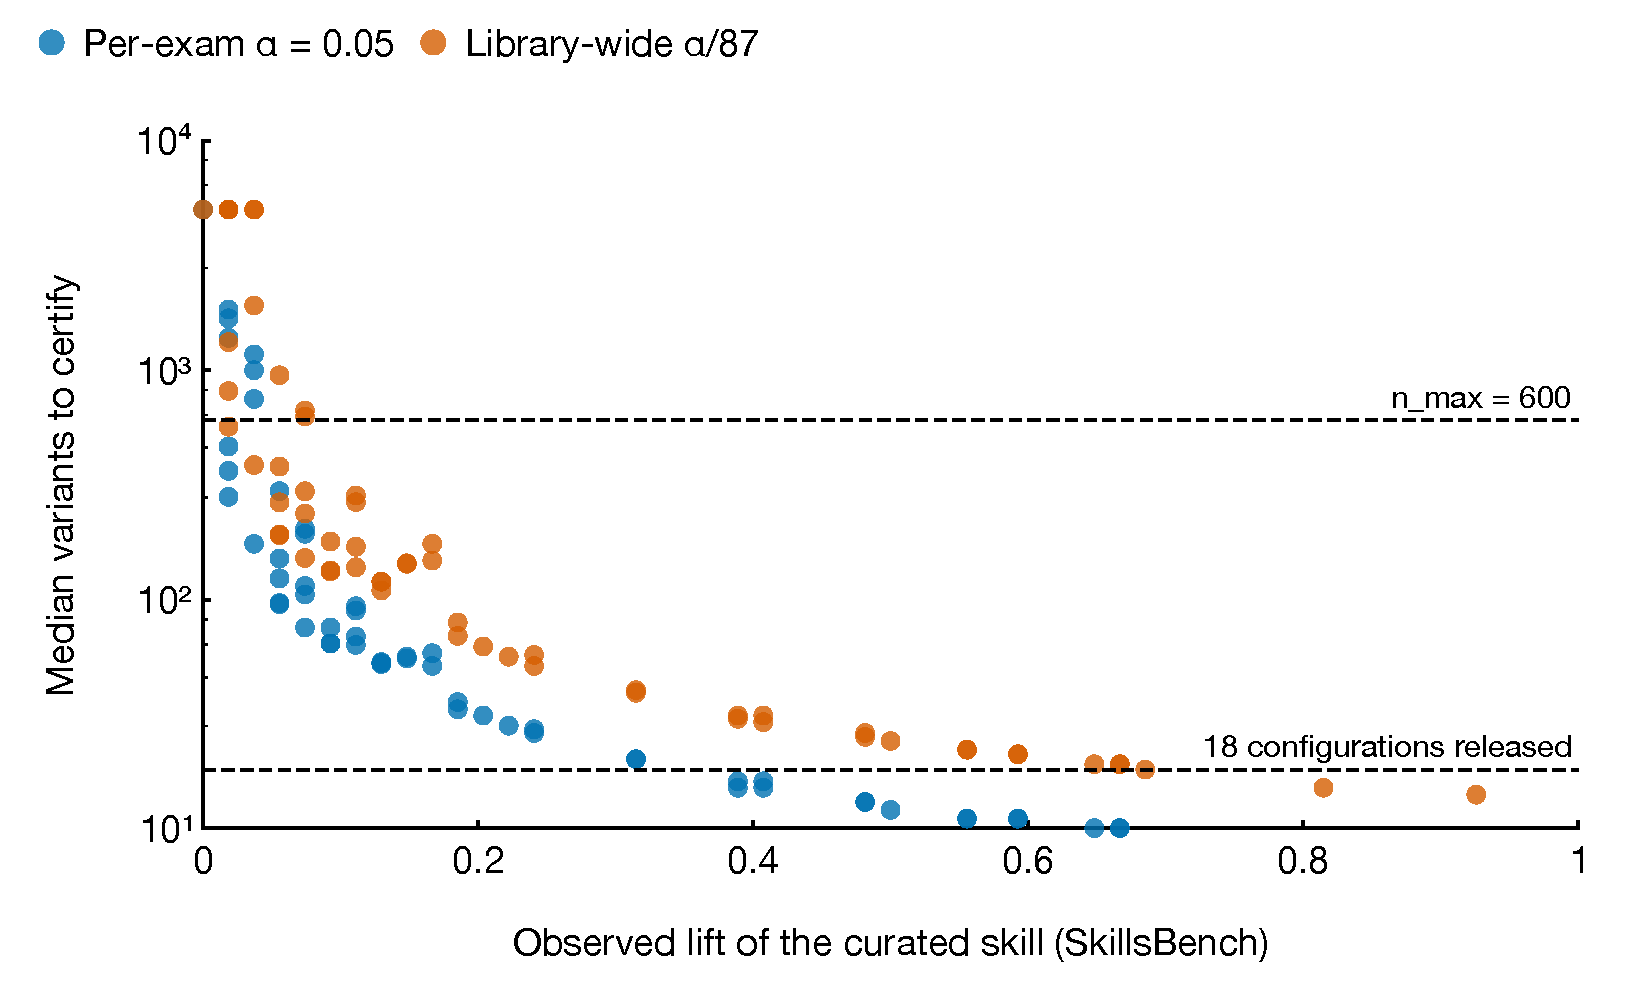
\includegraphics[width=0.48\linewidth]{F5_variants_needed.pdf}
\caption{Median variants needed to certify each SkillsBench curated skill with positive observed lift (\NSbPos{} skills), by resampling its released per-configuration differences (E9; 1{,}000 resamples per skill). Points at the top did not certify within 2{,}000 variants.}
\label{fig:need}
\end{figure}

\begin{figure}[!htb]
\centering
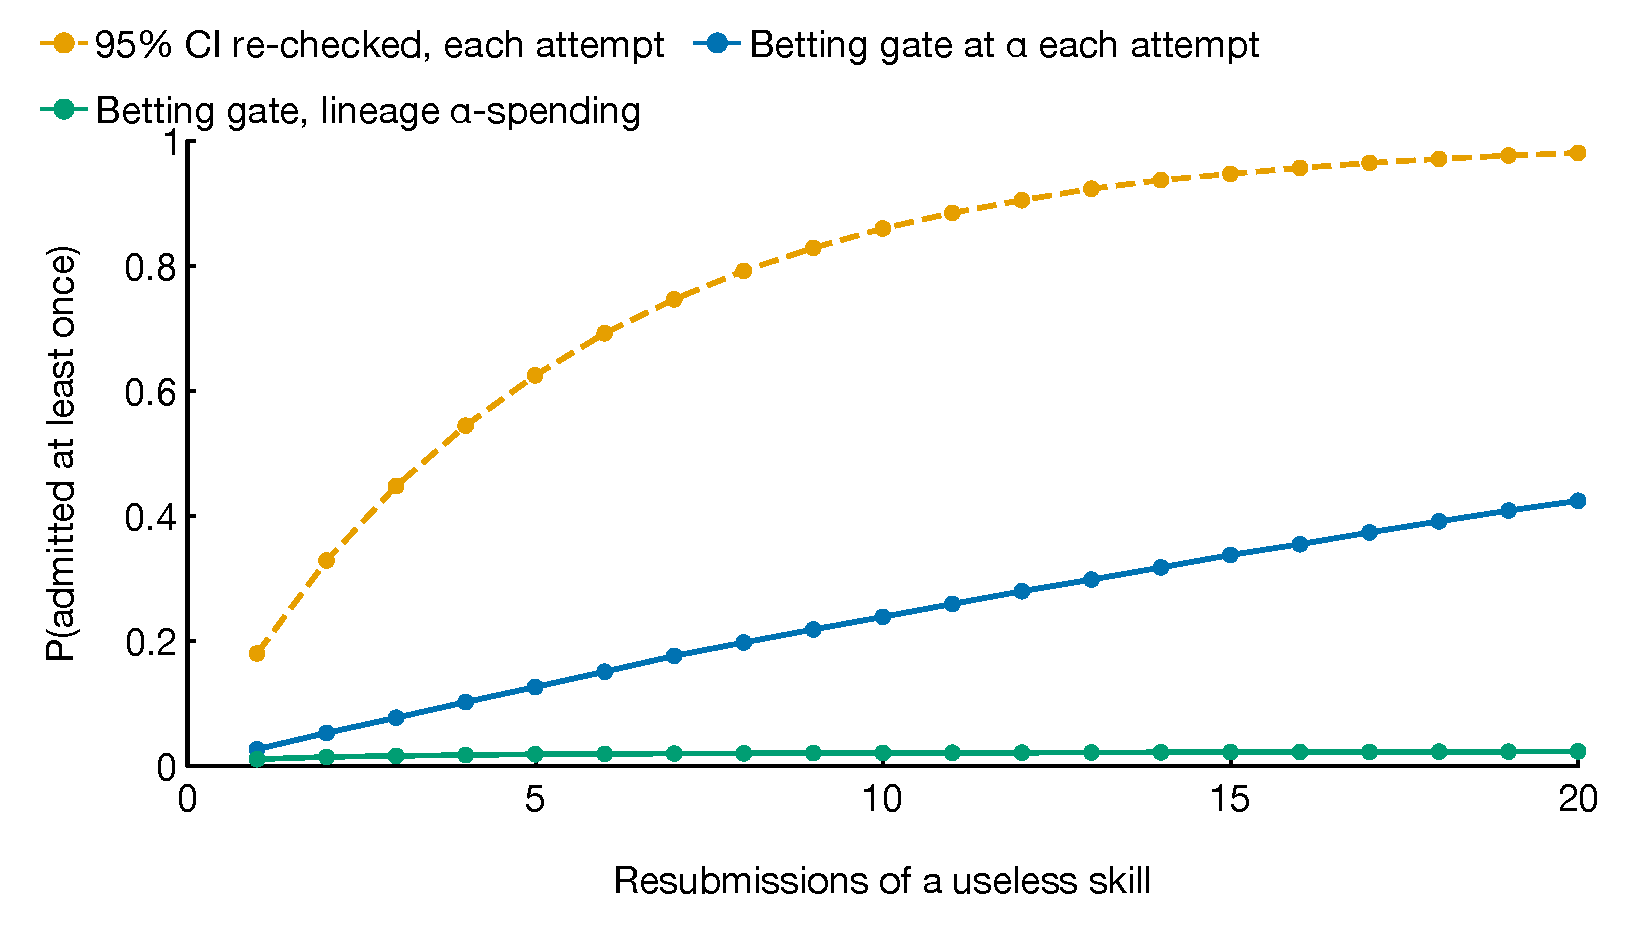
\includegraphics[width=0.48\linewidth]{F4_resubmission.pdf}
\caption{Probability that a useless skill ($\Delta=0$) has been admitted after $k$ resubmissions, each a fresh exam (E3).}
\label{fig:resub}
\end{figure}

\paragraph{Ten units (E8).} With the PrPl cap $c$ the wealth after $n$ units is at most $(1+c/2)^n$, so reaching $1/\alpha=20$ needs 14 units at $c=1/2$ (ten give at most \NSweMaxWealth) and all ten differences equal to 1 at $c=3/4$ (wealth \NSweMaxWealthHi; the largest any cell reached was \NSweObsWealth).

\paragraph{Fixed-sample library procedures and the theory checks (E10, E11).} E10 applies Benjamini-Hochberg, Benjamini-Yekutieli and Bonferroni at $\alpha=0.05$ to one-sided paired $t$-test and exact sign-flip $p$-values for the \NSbTasks{} SkillsBench skills, on all 18 configurations and on 200 random half-splits. On all 18 configurations, exact sign-flip tests certify \NFnSfBH{} skills under Benjamini-Hochberg, \NFnSfBY{} under Benjamini-Yekutieli and \NFnSfBonf{} under Bonferroni ($t$-tests: \NFnTBH, \NFnTBY{} and \NFnTBonf). Decided on nine configurations, Benjamini-Yekutieli certifies \NFnSplitTBY{} skills with $t$-tests and none with sign-flip tests, because with nine pairs the smallest exact sign-flip $p$-value, $1/512$, exceeds the Bonferroni threshold $0.05/87$; sign-flip tests with Benjamini-Hochberg certify \NFnSplitSfBH{} skills on average from nine configurations. E11 takes each of the \NThHelpful{} skills with positive released lift, uses its 18 per-configuration differences as $P$, computes $K_{\inf}$ by maximizing $g_P$, builds $Q^*$, and resamples 400 exams per skill at $\alpha=0.05$ without truncation or futility for the Kelly bet, PrPl with $c=1/2$, and aGRAPA with $c=1/2$ and $c=0.9$ (median $\NThAgrapaHiRatio\times$ the lower bound). The lineage checks resample 2000 exams of the median skill (\NThMedTask) at levels $\alpha q_k$ for three schedules. Attempt-count laws are truncated at 200 attempts. E12 checks Section~\ref{sec:theory}'s schedule results. It computes worst-case excesses over $\Pi_N$ for $N$ from 5 to 1{,}000, and certified intervals for $R(\Pi_N^\downarrow)$ for $N$ from 10 to 3{,}000 (width below $10^{-3}$ nats). It estimates $\mathbb E\,\mathrm{KL}(\pi\|\hat q)$ for the learned schedule of Theorem~\ref{thm:learned} from 4{,}000 draws of the counts, with $N=20$, $\epsilon=0.05$, three laws $\pi$ (geometric with mean 3, Zipf with exponent 2, uniform), $m$ from 0 to 1{,}000 and 0, 10 or 50 poisoned counts at the least likely attempt; every estimate is below the bound of part (b). For variants, it simulates 2000 exams of the median skill with the Kelly bet at 17 levels; expected variants grow linearly in $\log(1/a)$ with slope \NScSlope, against $1/K_{\inf}=\NScOneOverG$, and lineage costs are read off this curve.

\paragraph{Details of E14.} The matched-power runs use the default model at $r=1$, \PRepsPower{} replicates per cell, the SPRT with type-II error $\beta\in\{0.20,0.10,0.05,0.01\}$, the betting gate with futility margin truncated at $N_{\max}\in\{150,200,300,600\}$, and the fixed-$n$ test planned for 80\% to 99\% power. The moment fit searches a grid of $s_\theta$ from 0.5 to 5, $s_g$ from 0 to 3 and $\rho$ from 0 to 0.95, then a finer grid around the best point, matching each candidate's moments on $10^5$ simulated differences at the released lift and comparator rate with a relative squared-error loss. The fitted $\rho$ sits at the edge of the grid. E23 widens the grid ($s_g$ up to 5, $\rho$ up to 0.999): the fit keeps $s_\theta=s_g=2.25$, now in the interior, and moves $\rho$ to 0.999, again at the edge, with a loss of 0.0149 against 0.0160. The fitted-model costs move by at most 4\% (for example 166 against 170 expected variants at lift 0.10, $r=1$, $\kappa=0$), and the range over all sensitivity cells is 37 to 389 variants against 37 to 392, so no cost conclusion depends on where the grid stops. The correlated model draws $g_i=g+s_g(\kappa z_i+\sqrt{1-\kappa^2}z_i')$ with $\theta_i=s_\theta z_i$ and solves for $g$ so that $\Delta$ is exact; each cost cell uses 3{,}000 replicates. For the library procedure, each of the 87 skills gets 400 resampled exams of up to 2{,}000 variants at each of 25 levels from $\alpha$ down to $10^{-6}\alpha$; an exam at an e-LOND level uses the largest grid level not above it, which can only overstate the cost. Each of 1{,}000 random arrival orders updates the e-LOND rejection count with admissions within 600 variants. On the same grid, the Bonferroni level gives a median of \NRvLibBonf{} variants and the per-exam level \NRvLibPerExam, close to the \NSbMedNBonf{} and \NSbMedNAlpha{} of E9.

\paragraph{Level-tuned grid (E13).} For each of the \NThHelpful{} skills, E13 runs the grid exam of Theorem~\ref{thm:adaptive}, the Kelly bet, the same grid with $\rho=1/2$, the PrPl bet ($c=1/2$) and aGRAPA on 1{,}000 shared resampled sequences at the levels $\alpha q_1$ and $\alpha$, with the grid truncated at $\lambda_j\ge10^{-4}/m_0$ (truncation drops weight and so keeps validity). At level $\alpha q_1$ the grid needs fewer variants than aGRAPA for \NAgGridBeatsAgrapa\% of the skills, and every simulated cost lies below the bound. For the median skill, 1{,}500 sequences per level give $K_{\inf}\mathbb E[\tau]-L$ for 17 levels; the Kelly bet's excess is at most \NAgKellyExMax{} nats. Validity is checked with 4{,}000 sequences of 2{,}000 draws from each skill's least-favourable null $Q^*$: the mean rejection rate is \NAgMeanReject\%, at level \NAgLevelQone\%.

\paragraph{Reported lift.} The stopped estimate overstates the lift by \NEFourRelBiasFive\% at $\Delta=0.05$ and \NEFourRelBiasTen\% at $\Delta=0.10$. A fixed-$n$ test reported only when significant has the same problem (\NEFourBiasFixedFive\% at $\Delta=0.05$). At admission the anytime-valid lower bound averages at most \NEFourLcbMax{} points.

\begin{figure}[!htb]
\centering
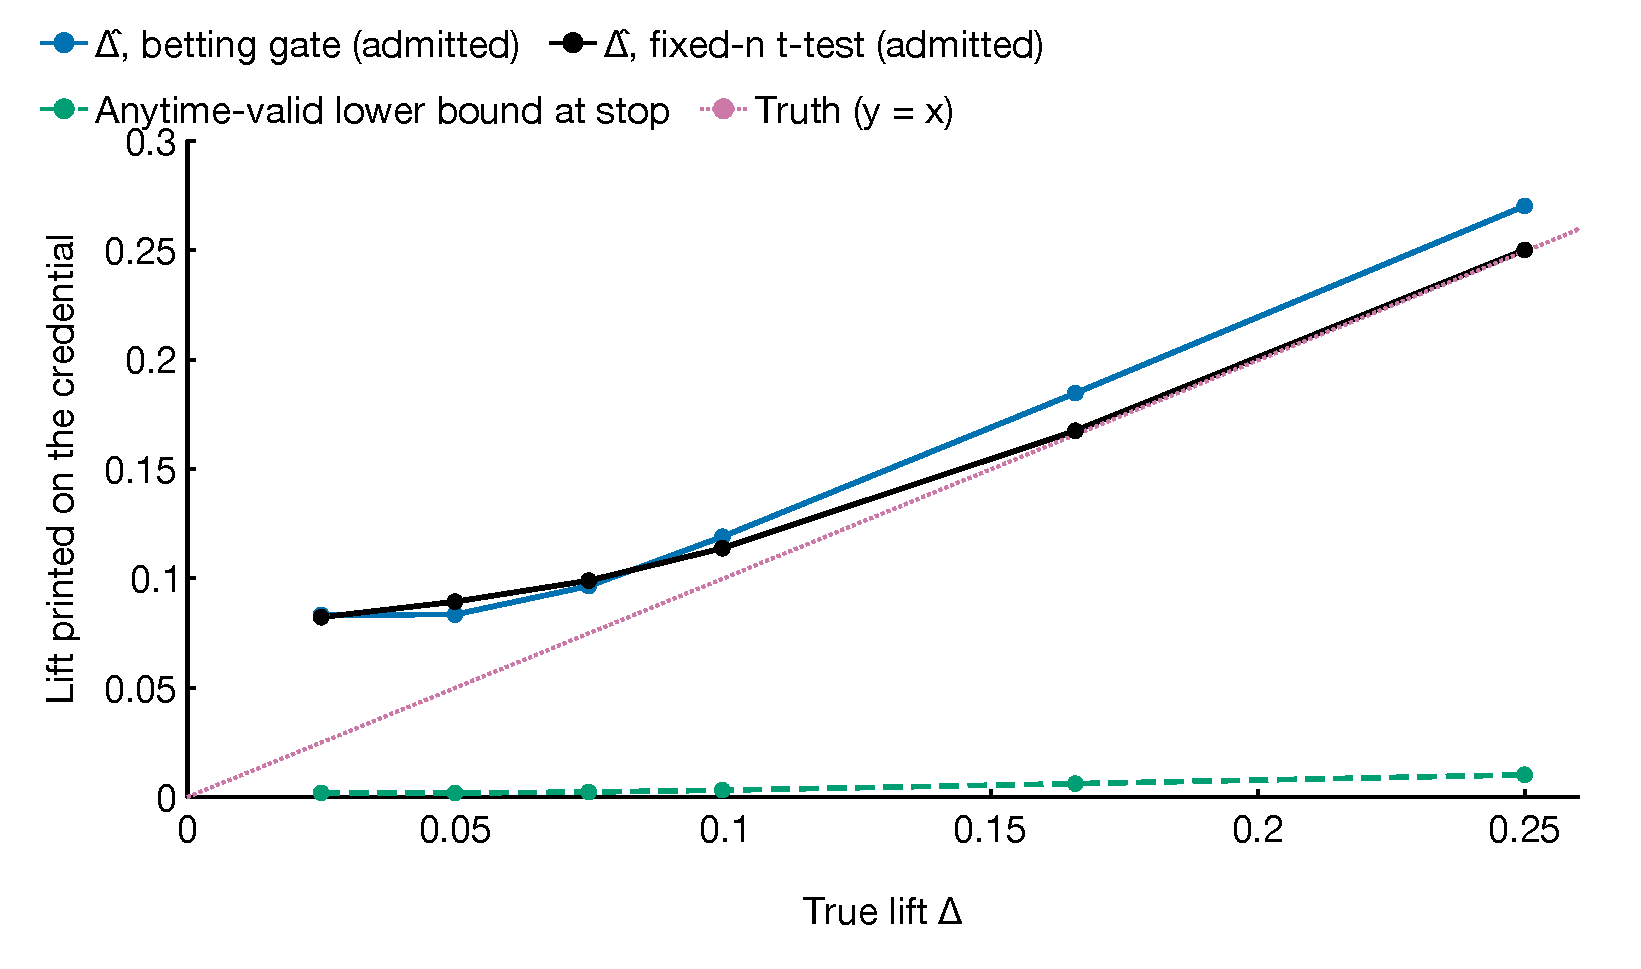
\includegraphics[width=0.48\linewidth]{F6_winners_curse.pdf}
\caption{Reported lift for admitted skills against the true lift (E4, 3{,}000 replicates per point).}
\label{fig:wc}
\end{figure}

\paragraph{Leakage and verification.} Tables~\ref{tab:leak} and~\ref{tab:verify} plant lookup tables covering 5\% of a \PGenSpace-instance generator space and flag a skill when its estimated coverage exceeds \PCoverMax\%. Normalizing separators and quotes catches spaced and split literals, and decoding base64 and hex runs catches encoded tables. On clean skills the false-positive rate was \NEsixFPLiteral\% for every detector; short numbers in honest text, such as status codes, gave a mean estimated coverage of \NEsixCleanCover\%. Our clean skills are templates, so this rate is a lower bound for real skills. For \NESevenN{} variants with \PTranscriptKB{}~kB transcripts (\NESevenMB{}~MB) the proctor's bookkeeping takes \NESevenProctor{}~s.

\begin{table}[!htb]
\centering\small
\caption{Leakage-check recall (\%) on planted tables, and false-positive rate on clean skills (E6).}
\label{tab:leak}
\begin{tabular}{lrrr}
\toprule
Skill (table covers 5\% of the space) & Literal & Normalized & Normalized + decoded \\
\midrule
Plain table & 100 & 100 & 100 \\
Spaced characters & 10 & 100 & 100 \\
Split string literals & 24 & 100 & 100 \\
Base64 blob & 0 & 0 & 100 \\
Hex blob & 0 & 0 & 100 \\
Generator code copied & 0 & 0 & 0 \\
Clean skills (false-positive rate) & 0 & 0 & 0 \\
\bottomrule
\end{tabular}

\end{table}

\begin{table}[!htb]
\centering\small
\caption{Credential cost (E7), median of three runs.}
\label{tab:verify}
\begin{tabular}{rrrrr}
\toprule
Variants $N$ & Transcripts (MB) & Proctor bookkeeping (s) & Verify (s) & Log bytes \\
\midrule
50 & 4 & 0.03 & 0.00 & 936 \\
100 & 8 & 0.05 & 0.01 & 936 \\
200 & 16 & 0.10 & 0.02 & 936 \\
400 & 32 & 0.21 & 0.04 & 936 \\
600 & 48 & 0.32 & 0.05 & 936 \\
\bottomrule
\end{tabular}

\end{table}

\paragraph{Live pilot.} We ran the full protocol once on a real agent: OpenHands with Claude Haiku~5.5 on \NPilotTasks{} SkillsBench tasks drawn by the committed rule from drand round \NPilotRound, three trials per arm, with both arms running concurrently. The model was changed by a logged amendment before any run; the amendment drew fresh secrets and a new beacon round. Two tasks errored in both arms (an agent crash and a sandbox that would not start) and were reported, not replaced, as pre-registered. On the \NPilotScored{} scored tasks the skills changed no pass count (mean $D=\NPilotDbar$, final wealth \NPilotWealth), so nothing was admitted. A separate run of the verifier opened both commitments, re-derived the task sample from the beacon, recomputed the decision from the logged transcripts and checked the signature; changing one recorded reward made it fail. The pilot cost about US\$2.5. % pilot/jobs/*/summary.json: 2.54
It demonstrates the protocol, not the effect of skills: four paired units are far too few (Section~\ref{sec:res-cost}).

\paragraph{Security screen (E15).} Helpfulness and safety are separate admission requirements \citep{wang2026skilltester}. We ran a static scanner, SkillSpector \citep{nvidia2026skillspector}, offline and without a language model, on the \NSecSkills{} skills shipped with the 87 SkillsBench tasks. It rated \NSecSafe{} safe, \NSecCaution{} caution and \NSecDNI{} do-not-install, the last in \NSecTasksFlag{} tasks, \NSecFlagHelpful{} of which have positive released lift. Risk score and released lift are unrelated (Spearman $\rho=\NSecRho$, $p=\NSecP$, 87 tasks). We scanned a clean export of the registered commit: a first scan of our working copy also flagged a skill for compiled bytecode that our own runs had left there. Each flagged skill was read three times by language models, each reading blind to the others and made from the skill files and scanner output alone: twice with Claude and once with GPT-5.5 (\texttt{gpt-5.5-2026-04-23}). All three readings found the same \NSecGenuine{} real concern among the \NSecFlagN{} flags, and none found another: a penetration-testing skill that instructs the agent to brute-force logins, collect private keys and add its own key to \texttt{authorized\_keys}, none of which its task needs. The readings rated the rest false positives or the result of files the scanner could not parse; the two Claude readings agreed on that category for \NSecCatAgree{} of \NSecFlagN{}, and GPT-5.5 called all of them false positives. A helpfulness certificate is therefore no evidence of safety, and the credential should carry the scan (tool version, rules, score) as a separate field.


\subsection{Live studies 1 to 3 in detail}
\label{app:live-detail}
\paragraph{On the benchmark.} We first ran the committed protocol on all \NLoTasks{} SkillsBench tasks with OpenHands and Claude Haiku~5.5 (API model identifier \texttt{claude-haiku-5-5}, runs on 15 and 16 November 2026), three trials per arm, in an order derived from drand round \NLoRound. The test asks whether the curated skills, taken as one library, help on average: $D_i$ is the per-task difference in passes divided by three, tested with the betting gate at $\alpha$ in the committed order. As committed, a task with an errored run in either arm was reported and excluded. \NLoExcluded{} tasks were excluded, for sandbox start-up refusals by the harness, agent-protocol and image failures, and a provider-side interruption during which model requests were rejected; \NLoMissing{} were never run because their environments request access to the host, which we did not grant. One logged amendment raised the budget after the first batch, whose results we had seen; a second reran two batches that the harness had refused as a whole. Continuing a betting test after seeing its path does not affect its validity (Proposition~\ref{prop:valid}), and both amendments are entries in the hash-chained ledger. On the \NLoScored{} scored tasks the mean difference was $\bar D=\NLoDbar$ (\NLoPos{} positive, \NLoNeg{} negative), the final wealth was \NLoWealth, short of $1/\alpha=20$, and the anytime-valid lower bound was \NLoLcb, so nothing was admitted. The verifier opened the commitment, re-derived the order from the beacon, recomputed the statistics from the \NLoRuns{} logged runs and checked the signature. It cost about US\$\NLoCost. The exclusions are not random: tasks whose images the harness refuses differ from those it runs.

\paragraph{On generated variants.} In the first family a variant is an access log of 60 to 90 lines generated from a 32-byte seed, and the task asks which client had the most server errors and how many. The logs follow two house conventions that cannot be inferred without documentation: the first field names the edge node that wrote the line, with the client in a trailing field, and status 599 records a client disconnect rather than a server error. The generator guarantees a unique answer, and in 95\% of variants the naive reading gives a wrong one.

Four skills were registered and hashed before the beacon round: a helpful skill that documents the conventions; a placebo of similar length with generic log-reading advice; a planted leak, which adds to the placebo a table of answers for 300 public example seeds; and a harmful skill that states wrong conventions. The model was Claude Haiku~5.5 (\texttt{claude-haiku-5-5}), called through the API with default settings on 16 November 2026. For each variant both arms answered the same log concurrently, and a pass is an exact match of client and count. The four exams ran in a committed order that includes a resubmission: the placebo, the leak and the harmful skill opened lineages A, B and C, and the helpful skill was submitted as the second attempt of lineage A. Exam $t$ ran at level $\min(\alpha_t,\alpha\gamma^{\text{lin}}_k)$ with e-LOND levels $\alpha_t$ (Proposition~\ref{prop:lineage}), with the betting gate, futility margin and $N_{\max}$ of Section~\ref{sec:gate}. Variant $j$ of exam $t$ used a seed derived from drand round \NLsRound, which did not exist when the commitment was logged. Before committing we ran five public variants per skill to check the harness (US\$\NLsCalCost); these were not scored, and we saw their results.

The leak table gave no lift (\NLsLeakWith{} passes with the skill, \NLsLeakWithout{} without): the exam variants came from seeds that did not exist when the skill was registered, so the table covered none of them. The harmful skill could not be told apart from the placebo, because the model rarely solved the task unaided (\NLsBasePct\% of variants without a skill) and so had little room to get worse; showing harm needs a family with a higher baseline. During the placebo exam a provider-side interruption rejected requests for a period; the \NLsPlacExcl{} affected pairs were reported and excluded, as committed, and the exam resumed at the next variant index. The study used \NLsPairs{} paired variants and cost US\$\NLsCost{} in API fees.

\paragraph{A second family and a resubmission attack.} We therefore ran a second committed study (drand round \NLsThreeRound) as a new registry history. Its family is an order export in CSV in which a channel code marks internal test orders that must be excluded from revenue, a convention the data do not reveal. The code changes the answer in about half the variants, so the model can succeed without documentation about half the time. A first version of this family, in which a numeric code marked refunds, was abandoned after calibration because the model guessed the code; both calibrations are in the ledger. Three skills were registered: a helpful skill that documents the code, a placebo of similar length, and a harmful skill that states a plausible but false pricing rule. The helpful skill was again submitted as the second attempt of the placebo's lineage. Finally, the placebo of the first study was resubmitted unchanged five times in one lineage, to exercise the level bookkeeping on a live model.

Without a skill the model passed \NLsBBasePct\% of the family's variants. The gate admitted the helpful skill after \NLsBHelpN{} variants (\NLsBHelpWith{} passes with the skill, \NLsBHelpWithout{} without, over \NLsBHelpRun{} variants run) and stopped the placebo for futility after \NLsBPlacN. The harmful skill was stopped for futility after only \NLsBHarmN{} variants (passes at the decision: \NLsBHarmTauWith{} with the skill, \NLsBHarmTauWithout{} without); the skill lowered the pass rate in every discordant variant (12 of 12; exact one-sided sign test after the fact on the \NLsBHarmRun{} variants run, $p=0.0002$). At \NLsBHarmN{} variants the anytime-valid upper bound on $\Delta$ was still \NLsBHarmUcb, above zero, so the gate refused the skill without certifying that it harms; a registry that wants to flag harmful skills needs a separate test with its own error budget. The five resubmissions ran at levels falling from \NLsResubLevelFirst{} to \NLsResubLevelLast{}, set in every case by the e-LOND term rather than the lineage term, as in most exams of E3b; \NLsResubAdmit{} were admitted, and at a per-exam level $\alpha$ without lineage spending \NLsResubAdmitPer{} would have been. With and without the placebo the model gave the same pass or fail on every variant, so each exam saw $D=0$ throughout and stopped for futility after \NLsResubNmin{} variants. Because the two arms never differed, any gate would have refused these attempts, so this part of the study is a check of the implementation, not evidence for lineage spending, whose error rate is a probability over histories (Section~\ref{sec:res-library}). The study cost US\$\NLsThreeCost, and its credential verified as in the first.

\paragraph{A second model.} Both studies used one closed model. To check that the gate's behaviour does not depend on it, we repeated them with an open-weight model from another family, Nemotron~3.5 Super VL (NVIDIA, released 15 October 2026; OpenRouter identifier \texttt{\NLnModel}), as two new registry histories committed before drand round \NLnRound{} on 17 November 2026. Everything but the model was kept: the skills, generators, prompts, graders, exam orders, levels and gate, all fixed by hash in the commitment. The model was called through OpenRouter with the provider pinned to the only endpoint that served the unquantized (bf16) weights and with fallbacks disabled, so that a response from any other provider would have counted as an error. Nemotron reasons at length before it answers, and its reasoning shares the token budget with the answer; in a smoke test on public variants, 6 of 20 answers were cut off at 8,000 tokens, so we committed a limit of \NLnMaxTok{} tokens for this model. Even so, \NLnCut{} of \NLnCalls{} calls (\NLnCutPct\%) reached the limit without a final answer and were graded as fails, as the pass rule requires. This is part of the model's measured behaviour under the committed settings; it lowers the pass rates the gate sees but not the validity of its decisions.

With Nemotron, every decision matched the one made with Haiku. In the second family the harmful skill lowered the pass rate in all \NLnBHarmDisc{} discordant variants (exact one-sided sign test after the fact, $p=\NLnBHarmSignP$), but the anytime-valid upper bound on $\Delta$ at the decision was still \NLnBHarmUcb, so the gate again refused the skill without certifying harm. Unlike Haiku, Nemotron did not always give the same result with and without the resubmitted placebo: \NLnResubDisc{} variants across the five attempts were discordant, so these exams saw nonzero differences. All five still stopped for futility, after \NLnResubNmin{} to \NLnResubNmax{} variants, and none would have been admitted at a per-exam level $\alpha$. Since a skill that helps one model can fail to help another \citep{yu2026masa,yang2026webdevskills}, a credential states the model under which the skill was admitted. The two studies used \NLnPairs{} paired variants; \NLnFailed{} calls failed and their pairs were excluded as committed. They cost US\$\NLnTotalCost{} in API fees, and both credentials verified.

\subsection{Study 4: published skills, selection and design}
\label{app:live-extra}
\paragraph{Shortlist and selection.} We searched public skill repositories for instruction-only skills (no bundled scripts) by authors other than the model providers, under an open licence, whose rules a program can check exactly. Three were shortlisted and ranked before any call, each pinned to a commit and a SHA-256 hash checked on load: \texttt{newsroom-style} by Joe Amditis (AP style; MIT), \texttt{commit} by Sentry (commit messages; Apache-2.0) and \texttt{apa7} by Kalaris Labs (APA~7; MIT). The selection rule, the window $[0.05,0.40]$ and the limit of one widening of the shortlist were fixed in the design document before calibration. Table~\ref{tab:s4cal} gives every calibration; their transcripts are in the ledger.

\begin{table}[tb]
\centering\small
\caption{Public calibrations for study 4 (20 variants per arm, seeds public, not scored). Passes with / without the skill. Selection used the Haiku lift only.}
\label{tab:s4cal}
\begin{tabular}{lllrrr}
\toprule
Skill & Model & Role & Published skill & Placebo & Lift \\
\midrule
AP style & Haiku & study 4b & \NCalFourBRealWith{} / \NCalFourBRealWithout & \NCalFourBPlacWith{} / \NCalFourBPlacWithout & \NCalFourBLift \\
Sentry commit & Haiku & study 4c & \NCalFourCRealWith{} / \NCalFourCRealWithout & \NCalFourCPlacWith{} / \NCalFourCPlacWithout & \NCalFourCLift \\
APA~7 & Haiku & study 4 (selected) & \NCalFourRealWith{} / \NCalFourRealWithout & \NCalFourPlacWith{} / \NCalFourPlacWithout & \NCalFourLift \\
APA~7 & Nemotron & study 4 & \NCalNFourRealWith{} / \NCalNFourRealWithout & \NCalNFourPlacWith{} / \NCalNFourPlacWithout & \\
\bottomrule
\end{tabular}
\end{table}

\paragraph{Task families.} In the AP family a variant is a set of reporter's notes written in non-AP form, and a brief passes if every graded item (dates, times, counts, ages, money, ``over'', attribution verbs) takes the form the skill prescribes. In the commit family a variant is a set of change notes, and a message passes if its header, type, subject, line lengths, breaking-change marker, issue footer and omission of a customer's contact details follow the skill. In the APA family a variant is a journal-article record with 1 to 30 authors, a title in title case and a DOI in a non-URL form; a pass requires the exact reference-list entry (including sentence-case title, en dash in the page range, \texttt{https://doi.org/} form and the rule for 21 or more authors, with the APA manual's punctuation ``nineteenth author, . . . final author'', which the skill states only as ``an ellipsis'') and the exact parenthetical citation, after a fixed normalization of whitespace, markdown emphasis and quotation marks. Each placebo is general advice on the same activity (news writing, commits, academic writing) of matched length, with none of the graded rules. In the AP family that was not enough to make the placebo inert. With it Haiku wrote ``over'' for ``more than'' in \NLsFourBPlacOverWith{} of \NLsFourBPlacOverN{} briefs that needed it (\NLsFourBPlacOverWithout{} without) and money in AP form in \NLsFourBPlacMoneyWith{} of \NLsFourBPlacMoneyN{} (\NLsFourBPlacMoneyWithout{} without). On Nemotron the placebo moved the same rules: ``over'' in \NLnFourBPlacOverWith{} of \NLnFourBPlacOverN{} briefs (\NLnFourBPlacOverWithout{} without) and money in \NLnFourBPlacMoneyWith{} of \NLnFourBPlacMoneyN{} (\NLnFourBPlacMoneyWithout{} without). Without the placebo the models almost never produced these forms. A control that cannot help must come from an unrelated activity; a placebo from the same activity tests whether the specific rules add to general advice. The commit and APA placebos keep the published skill's name in their header (\texttt{commit}, \texttt{apa7}); the AP placebo is named \texttt{newsroom-craft}, so the model saw a different name in that study only. Titles in the APA family are filled from fixed templates and are sometimes ungrammatical (``a experimental study''); both arms see the same record.

\paragraph{Power plan.} The plan simulated the grid-bet exam at the paired outcome law estimated from the Haiku calibration and at a conservative law, and chose the first design (placebo first, then real skill first; $N_{\max}$ from 600 to 1800) with conservative power at least $0.80$. The first version of the conservative law lowered the lift by one standard error but ignored variants in which the skill turns a pass into a fail; the placebo calibration showed such variants occur, so before commitment we amended it to add the placebo's discordance rate (\NPowNoise{} per side) to both sides. Conservative power fell from \NPowConsVone{} to \NPowCons, the design was unchanged, and both versions are in the record. Studies 4b and 4c, with large calibration lifts, used the design of studies 2 and 3 without a simulation.

\paragraph{Excluded pairs.} Only the Nemotron arm of study 4 lost pairs: all \NLnFourPlacExcl{} exclusions in its placebo exam (of \NLnFourPlacRun{} pairs run) and all \NLnFourRealExcl{} in its skill exam (of \NLnFourRealRun) were caused by rate-limit errors (HTTP 429) from the pinned provider. Failed calls were \NLnFourPlacFailWith{} with the skill and \NLnFourPlacFailWithout{} without it in the placebo exam, and \NLnFourRealFailWith{} and \NLnFourRealFailWithout{} in the skill exam. The committed rule excludes a pair whose call fails in either arm after retries. A rate-limit error is returned before the model produces anything, so exclusion cannot depend on the outcome the failed call would have had, and the decision uses the remaining pairs in their original order. In the same arm \NLnFourCut{} answers reached the token limit and were graded as fails.

\paragraph{Deviations from the protocol, and why they do not affect the decisions.} Three things did not go as written; each is in the ledger with the logs of the failed attempts.

\emph{(i) Wrong labels.} A substitution error in the script that generated the runners of studies 4b and 4c made the descriptive label of their Nemotron arms read ``4bbN'' and ``4ccN''. The label is text only: the ledger entry kinds, seeds, transcript folders and all hashed objects are correct. We left it as committed, because changing it would change the hash the verifier checks.

\emph{(ii) A run that stopped before it started.} The first attempt to run the Nemotron arms of 4b and 4c stopped before writing any transcript, because the transcript folder did not exist. The rerun regenerated the same seeds; no outcome of the first attempt was recorded or seen.

\emph{(iii) An early reveal.} In the Nemotron arm of study 4 the exams were first started before the committed beacon round existed, and a build step run by mistake afterwards logged the reveal of the committed secret at 16:05:45 UTC, nine seconds before beacon round 34071530 was published and before any exam ran. The secret keeps the hidden variants unknown both to whoever chooses the skills, generator and grader and to a submitter during the exam, on which resubmission-proofness relies. Neither role was compromised: the variant seeds hash the secret with the beacon, so they could not be computed before the round existed; both attempts of the lineage and the generator, prompt, grader and plan were fixed by hash in a commitment logged two minutes earlier; and the ledger was private. The exams then ran under the same commitment, and each decision follows mechanically from the transcripts. The ledger shows both, identical, reveal entries. The verifier's checks do not test that a reveal follows the close of the exams, so a passing verification does not attest it. Our runners did not refuse an early reveal; the released code will, and the committed runners stay unchanged so that their hashes verify.

\paragraph{Study 5: an externally built family (E25).} The generator is Google DeepMind's \texttt{mathematics\_dataset} 1.0.1 \citep{saxton2019analysing} (Apache-2.0), installed from PyPI and called unmodified in a pinned environment. A variant is a (module, regime, seed) triple; only modules whose draws do not depend on earlier draws were eligible (35 training modules in the hardest regime and 14 extrapolation modules). The selection rule, written before any model call on the family, ran 16 public-seed questions per eligible module through Haiku without a skill and kept the modules with a pass rate in $[0.30,0.60]$, at most one per area, closest to $0.45$ first. Two qualified, from different areas: primality testing (7 of 16) and division of large numbers (9 of 16). A variant's module is chosen by its seed with probability $1/2$ each. The model must put its answer inside \texttt{<answer>} tags; a pass is an exact match after normalisation, or equality as exact rationals.

The three published skills, \texttt{Math.Skill}, \texttt{math-teacher} and \texttt{math-help}, come from three public repositories, are MIT-licensed, and were used byte for byte at the commits pinned in the release, which names the repositories. We wrote the placebo (general work habits, no mathematical method) and the harmful skill (a primality screen that divides only by 2, 3, 5, 7 and 11, with composite numbers given as prime examples, and division answers as six-significant-figure decimals where the generator asks for exact fractions), both matched in length. The paired calibration ran 20 public-seed variants per skill with Haiku; every calibrated lift was negative (from $-0.05$ for the placebo to $-0.30$ for the harmful skill), so the power plan found no cap that reaches its target and the rule fixed in advance set $N_{\max}=600$. The Nemotron study used the same plan and the same exam order, levels and seed derivation, in its own registry history (drand rounds \NLsFiveRound{} and \NLnFiveRound). Nemotron ran with a 16{,}000-token limit and reached it in \NLnFiveCutPct\% of its answers over the study; Haiku reached its limit in \NLsFiveCutPct\% of its answers, most often in the \texttt{Math.Skill} exam with the skill (\NLsFiveSkillCutWith{} of \NLsFiveSkillRun). Four pairs of the Nemotron harmful exam were excluded for API failures after retries, under the committed rule.

\emph{Deviations.} (i) \emph{Grader.} The grader frozen before calibration (v1) failed mathematically correct answers whose terms were in another order and multiple-choice answers that gave the right letter with its value. We changed it (v2: SymPy equality for arithmetic expressions in integers and square roots, and the leading letter for multiple choice) after the no-skill calibration and before any skill was run, so the change cannot favour a skill, and re-graded the calibration offline with no new calls; both versions are in the release. Module selection used the v2 rates. (ii) \emph{Restarts.} The first Haiku run stopped with HTTP 425 because the committed beacon round had not yet been published, before any variant was drawn. The first Nemotron run failed on its first chunk because its transcript folder did not exist; nothing was written or logged, and the rerun started exam 1 from pair 0 with the same committed seeds, as for studies 4bN and 4cN. (iii) \emph{Labels.} The docstring of the committed runner was carried over from study 4 and names the old commands and budget; the values that apply are in the code and the committed parameters. Every decision recomputes from the ledger and transcripts with the released verifier.
